\section{Evaluation and Discussion}\label{sec:performance}

In this section we evaluate the performance of
the implementation of our method
on a real collection of X images of Y size.
\begin{edit}
TODO
\end{edit}

\subsection{Generalization across image categories and sizes}
\label{sec:growing_db}

In the preceding sections, we determined that for an image sized $500\times 500$, a $25\times 25$ patch size with a $T=0.01$ patch distance threshold is appropriate since compression savings are properly balanced against artifacts introduced during image reconstruction. For further experiments, we scale down the image size to $100\times 100$ and the patch size to $5\times 5$, accordingly, maintaining the patch:image size ratio. Note that the distance threshold still applies as it is independent of patch size. The reduction in image size allows us to consider larger experiments on databases of image thumbnails. 

In fig. \ref{fig:bigsize} we consider the growth of the patch dictionary as we add 2K images to our database. We add images from different categories, and observe a slight change in dictionary growth rate for every new category added. Although there is some variation across categories, the overall compression is $18.95\%$ per image, demonstrating generalization across categories.

 \begin{figure}
\hspace{-5mm}
%\centering
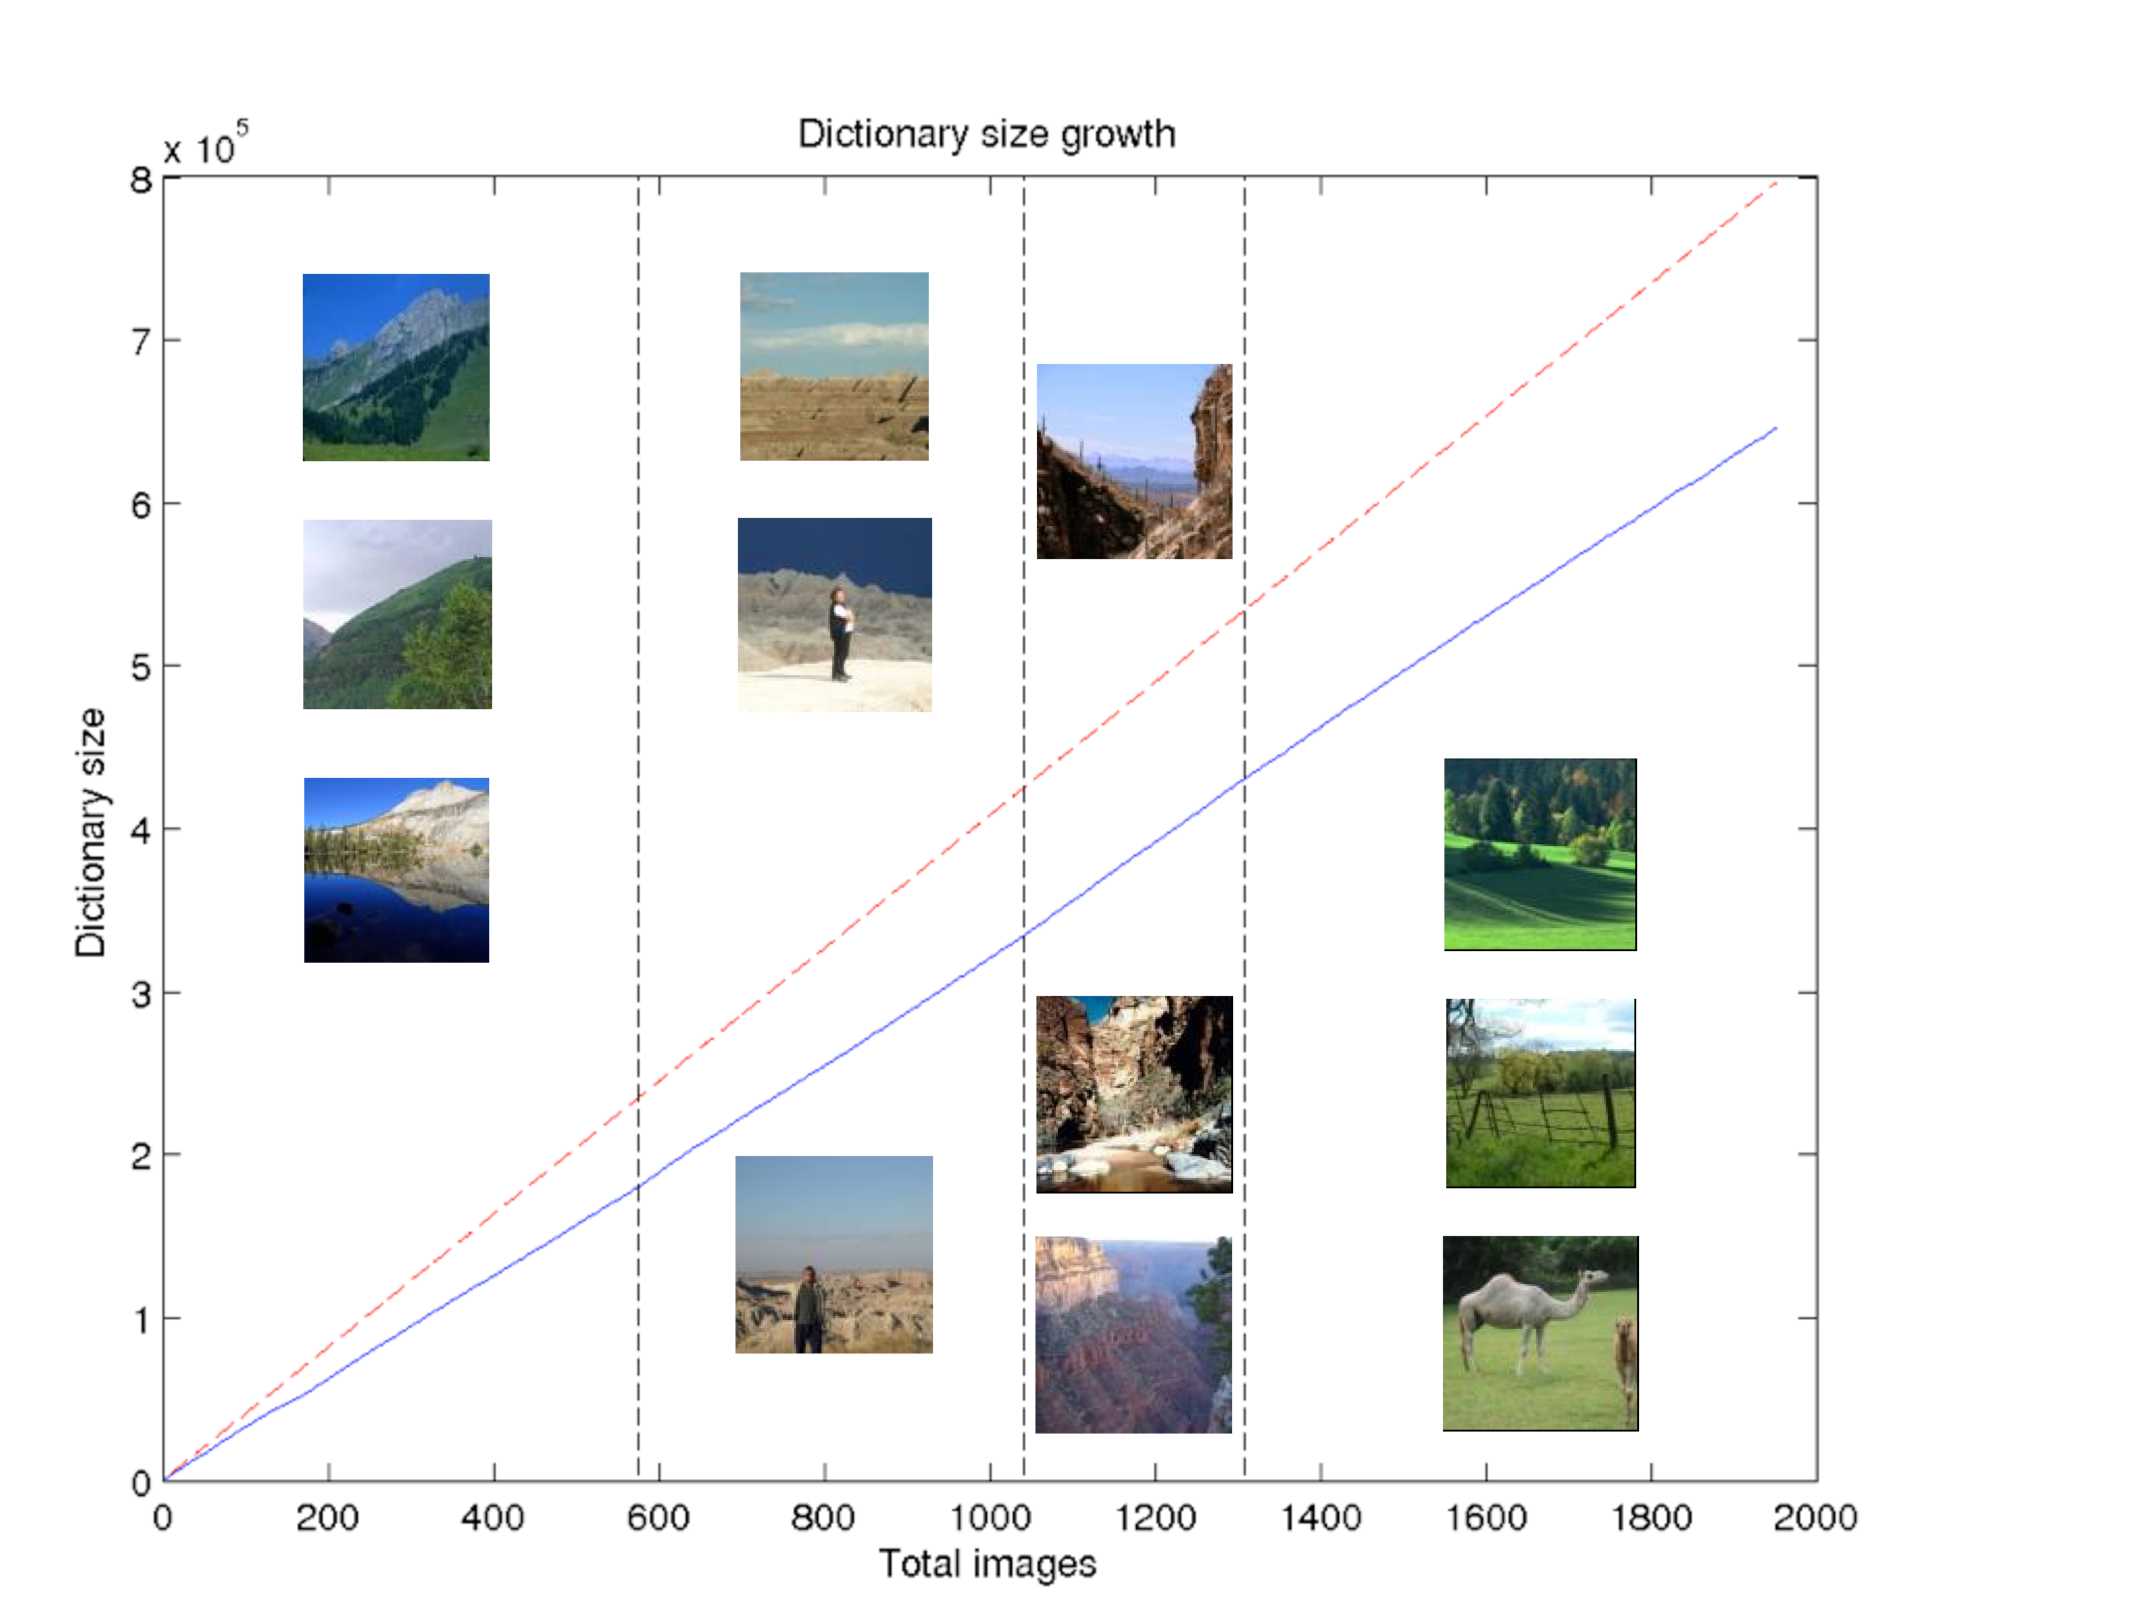
\includegraphics[width=1.3\linewidth]{Figures/multiscenes.pdf}
\caption{A patch dictionary constructed from $5\times 5$ patches from $100\times 100$ images, with a $T=0.01$ patch distance threshold, obtains an average compression of $18.95\%$ per image. The average number of new patches added per image is $330.70$ with a total dictionary size of $645,534$ patches representing 1952 images. The black dotted vertical lines mark the addition of new image categories, (left to right) mountain (with dictionary growth rate 312.96, equivalent to compression of $21.76\%$ per image), badlands (growth rate 330.50, compression $17.38\%$), canyon (growth rate: 360.61, compression $9.85\%$), and pasture (growth rate: 334.11, $16.47\%$). A few image samples from the 4 categories are included.  Note that for this growth rate, storing image patches will always take less space than storing the entire image, since $c < c'$.}
\label{fig:bigsize}
\end{figure}

Not all image content is amenable to the same type of compression. For some types of images, particularly where there is a lot of spatial structure (e.g. indoors scenes with objects and parts), compression artifacts are much more noticeable and thus distance thresholds should be more stringent. An interesting extension that is beyond the score of this paper would be to have a content-aware distance threshold (self-adjusting to content type such as indoor vs outdoor/natural).

For our database system, compression works for both indoor and outdoor images. In outdoor images, a lot of the compression savings come from accounting for the homogeneous sky patches (which may take up a large portion of the image). Although indoor images often contain many more objects and are more cluttered than outdoor images, they contain large homogenous regions corresponding to the walls and ceilings of rooms, which can surprisingly compress better than some outdoor images (walls may be more homogeneous than the sky). Thus, our compression approach generalizes to different types of scenes.

\begin{edit}
If time allows, insert sample image reconstructions from different categories 
\end{edit}


\subsection{Quantitative}\label{ssec:quant}
\begin{edit}
TODO
\end{edit}


\subsection{Qualitative}\label{ssec:qual}
\begin{edit}
TODO
\end{edit}
